% $Header: /cvsroot/latex-beamer/latex-beamer/solutions/conference-talks/conference-ornate-20min.en.tex,v 1.6 2004/10/07 20:53:08 tantau Exp $

\documentclass{beamer}

% This file is a solution template for:

% - Talk at a conference/colloquium.
% - Talk length is about 20min.
% - Style is ornate.



% Copyright 2004 by Till Tantau <tantau@users.sourceforge.net>.
%
% In principle, this file can be redistributed and/or modified under
% the terms of the GNU Public License, version 2.
%
% However, this file is supposed to be a template to be modified
% for your own needs. For this reason, if you use this file as a
% template and not specifically distribute it as part of a another
% package/program, I grant the extra permission to freely copy and
% modify this file as you see fit and even to delete this copyright
% notice. 


\mode<presentation>
{
  %\usetheme{default}
  \usetheme{Pittsburgh}
  %\usecolortheme{crane}
  % or ...

  \setbeamercovered{transparent}
  \setbeamerfont{small}{size=\small}
  % or whatever (possibly just delete it)
}


\usepackage[english]{babel}
% or whatever

\usepackage[latin1]{inputenc}
% or whatever

\usepackage{times}
\usepackage[T1]{fontenc}
% Or whatever. Note that the encoding and the font should match. If T1
% does not look nice, try deleting the line with the fontenc.


\title[]
{Combining Bidirectional Translation and Synonymy for Cross-Language Information Retrieval}

\author[] % (optional, use only with lots of authors)
{Ruey-Cheng Chen}
% - Give the names in the same order as the appear in the paper.
% - Use the \inst{?} command only if the authors have different
%   affiliation.

\institute % (optional, but mostly needed)
{
  Institute of Information Science, Academia Sinica, Taiwan
}
% - Use the \inst command only if there are several affiliations.
% - Keep it simple, no one is interested in your street address.

\date[] % (optional, should be abbreviation of conference name)
{Survey of SIGIR'06}

% - Either use conference name or its abbreviation.
% - Not really informative to the audience, more for people (including
%   yourself) who are reading the slides online

\subject{Theoretical Computer Science}
% This is only inserted into the PDF information catalog. Can be left
% out. 

% If you have a file called "university-logo-filename.xxx", where xxx
% is a graphic format that can be processed by latex or pdflatex,
% resp., then you can add a logo as follows:

% \pgfdeclareimage[height=0.5cm]{university-logo}{university-logo-filename}
% \logo{\pgfuseimage{university-logo}}



% Delete this, if you do not want the table of contents to pop up at
% the beginning of each subsection:
\AtBeginSubsection[]
{
  \begin{frame}<beamer>
    \frametitle{Outline}
    \tableofcontents[currentsection,currentsubsection]
  \end{frame}
}


% If you wish to uncover everything in a step-wise fashion, uncomment
% the following command: 

%\beamerdefaultoverlayspecification{<+->}


\begin{document}

\begin{frame}
  \titlepage
\end{frame}

\begin{frame}{Outline}
  \tableofcontents
  
  % You might wish to add the option [pausesections]
\end{frame}


% Structuring a talk is a difficult task and the following structure
% may not be suitable. Here are some rules that apply for this
% solution: 

% - Exactly two or three sections (other than the summary).
% - At *most* three subsections per section.
% - Talk about 30s to 2min per frame. So there should be between about
%   15 and 30 frames, all told.

% - A conference audience is likely to know very little of what you
%   are going to talk about. So *simplify*!
% - In a 20min talk, getting the main ideas across is hard
%   enough. Leave out details, even if it means being less precise than
%   you think necessary.
% - If you omit details that are vital to the proof/implementation,
%   just say so once. Everybody will be happy with that.

\section<presentation>*{Reference}

\frame{
  \frametitle{Reference}
  \begin{thebibliography}{10}
%--------------------------------------------------
%     \beamertemplatebookbibitems
%     \bibitem{Author1990}
%       A.~Author.
%       \newblock {\em Handbook of Everything}.
%       \newblock Some Press, 1990.
%-------------------------------------------------- 
    \beamertemplatearticlebibitems
    \bibitem{Wang06}
      {\bf Jianqiang Wang and Douglas W. Oard} \\
      {\em College of Information Studies and UMIACS} \\
      {\em University of Maryland} \\

      \newblock Combining bidirectional translation and synonymy for cross-language information retrieval.
      \newblock In {\em Proceedings of the 29th Annual International ACM SIGIR Conference on Research and Development in information Retrieval (SIGIR '06)}. pages 202-209, ACM Press, 2006.
  \end{thebibliography}
}

\section{Background}

\frame{
  \frametitle{Motivation}
  \begin{block}{Cross-Language Meaning Matching}
    \begin{itemize}
    \item High flexibility
    \item Approximation to meaning
    \item Subsumption for existing approaches to query and document translation
    \item Effectiveness
    \end{itemize}
  \end{block}
}

\frame{
  \frametitle{Translation in CLIR}
  \begin{block}{Document Translation}
    \begin{itemize}
    \item To approximate what would have happened if the authors had written in the query language
    \item Limited context with high computational costs
    \end{itemize}
  \end{block}
  \begin{block}{Query Translation}
    \begin{itemize}
    \item To approximate what would have happened if the search had expressed their query in the document language
    \item Limited context with short queries
    \end{itemize}
  \end{block}
}

\frame{
  \frametitle{Bidirectional Translation}
  \begin{block}{The First Effort [McCarley99]}
    \begin{itemize}
    \item Merging two ranked lists generated using query and document translation, respectively
    \item Significant improvements in mean average precision (MAP)
    \item Similar result obtained by [Braschler04, Kang04]
    \end{itemize}
  \end{block}
}

\section{Matching Meaning}

\frame{
  \frametitle{Formalization}
  \begin{block}{Probabilistic Structured Queries (PSQ) [Darwish03]}
    $TF(e,D_k) = \sum_{f_i}\limits p(f_i \mid e) \times TF(f_i,D_k)$ \\
    $DF(e) = \sum_{f_i}\limits p(f_i \mid e) \times DF(f_i)$
  \end{block}

  \begin{block}{Our Approach}
    $TF(e,d_k) = \sum_{f_i}\limits p(e,f_i) \times TF(f_i,d_k)$ \\
    $DF(e) = \sum_{f_i}\limits p(e,f_i) \times DF(f_i)$
  \end{block}
}

\frame{
  \frametitle{Idea}
  \begin{block}{Assumption}
    The searcher's choice of meaning for term $e$ is independent of the author's choice of meaning for term $f$
  \end{block}
  \begin{block}{General Form of $p(e,f)$}
    Generalizing to any pair of words $e$ and $f$:
    \begin{equation}
    p(e,f) \sim \sum_{s_j}\limits p(s_j \mid e) \times p(s_j \mid f)
    \end{equation}
    where $p(e,f)$ is the probability that term $e$ and term $f$ have the same meaning,
    $p(s_j \mid e)$ is the probability that term $e$ has the meaning $s_j$,
    and $p(s_j \mid f)$ is the probability that term $f$ has the meaning $s_j$,
  \end{block}
}

\frame{
  \frametitle{Idea (cont'd)}
  \begin{figure}
    \centering
    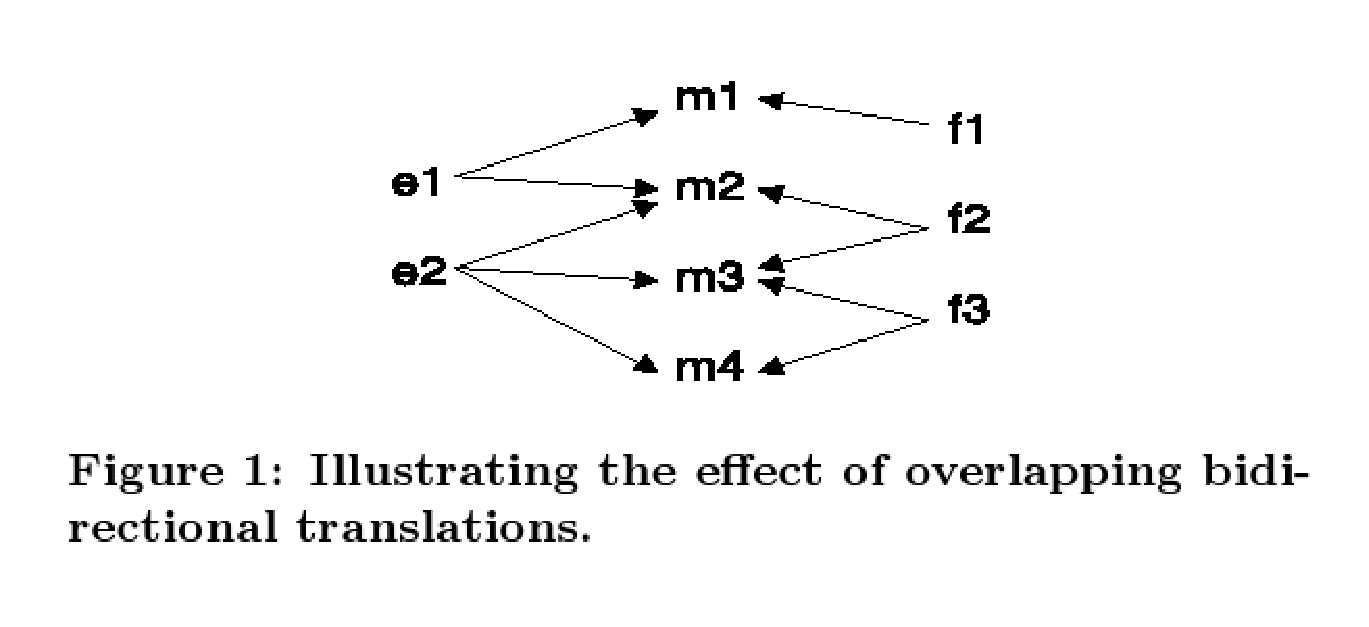
\includegraphics[width=\columnwidth]{fig/fig1}
  \end{figure}
}

\frame{
  \frametitle{Methods}
  \begin{itemize}
  \item Full Aggregated Meaning Matching (FAMM)
  \item Derived Aggregated Meaning Matching (DAMM)
  \item Individual Meaning Matching (IMM)
  \item Probabilistic Structured Queries (PSQ)
  \end{itemize}
}

\frame{
  \frametitle{Method 1 and 2: FAMM and DAMM}
  \begin{block}{Idea}
    \begin{description}
    \item[FAMM] Cross-language synset alignments are available from sources (e.g., \textit{EuroWordNet})
      \begin{equation}
      p(e,f) = \sum_{s_j}\limits p(s_j \mid e) \times p(s_j \mid f)
      \end{equation}
    \item[DAMM] Synset alignments are not available, so the alignments are built by employing a greedy algorithm
      \begin{equation}
      p(e,f) = p(s_j \mid e) \times p(s_j \mid f)
      \end{equation}
    \end{description}
  \end{block}
}

\frame{
  \frametitle{Cross-Language Synset Alignment}
  \begin{block}{Sub-problems}
    \begin{itemize}
    \item Mapping words across languages
    \item Mapping words in each language into monolingual synsets
    \item Aggregating the word-to-word mappings to produce word-to-synset mappings
    \item Aligning the resulting synsets
    \end{itemize}
  \end{block}
}

\frame{
  \frametitle{Cross-Language Synset Alignment (cont'd)}
  \begin{block}{Monolingual Synset}
    Monolingual synsets can be obtained from \textit{WordNet} or from statistical word-to-word translation model:
    \begin{equation}
    p(f_j,f) \sim \sum_{i=1}^n\limits p(e_i \mid f) \times p(f_j \mid e_i)
    \end{equation}
  \end{block}
  \begin{block}{Word-to-Synset Mapping Model}
    \begin{enumerate}
    \item Compute $p(s_j \mid e) = \sum_{f_i \in s_j} p(f_i \mid e)$, and rank all $s_j$ in 
    decreasing order of $p(s_j \mid e)$;
    \item Select Synset $s_j$ with the largest aggregate probability
    and remove all of its terms from every synset and iterate.
    \end{enumerate}
  \end{block}
}

\frame{
  \frametitle{Word-to-Synset Mapping}
  \begin{figure}
    \centering
    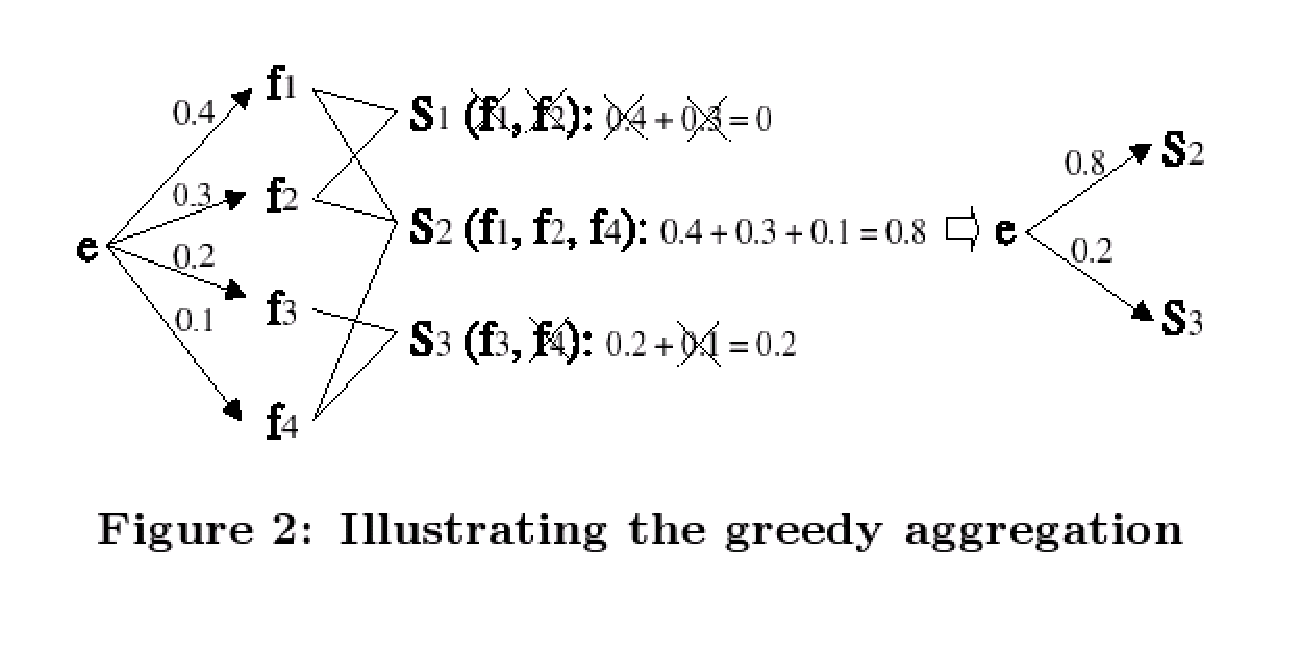
\includegraphics[width=\columnwidth]{fig/fig2}
  \end{figure}
}

\frame{
  \frametitle{Method 3 and 4: IMM and PSQ}
  \begin{block}{Idea}
    \begin{description}
      \item[IMM] Assuming that each term encodes a unique meaning, we get:
	\begin{equation}
	p(e,f) = p(e \mid f) \times p(f \mid e)
	\end{equation}
      \item[PSQ] Assuming a uniform distribution for $p(e \mid f)$ across all $y$, we get:
	\begin{equation}
	p(e,f) = p(f \mid e)
	\end{equation}
    \end{description}
  \end{block}
}

\section{Experiments}

\frame{
  \frametitle{Setup}
  \begin{block}{Test Collection}
    \center
    \begin{tabular}{|l|c|c|}
      \hline
      Test collection from & CLEF'01-03 & TREC-5,6 \\
      \hline
      Query language & English & English \\
      Document language & French & Chinese \\
      \# of search topics & 151 & 54 \\
      \# of documents & 87,191 & 139,801 \\
      Avg. \# of rel. docs per topic & 23 & 95 \\
      \hline
    \end{tabular}
  \end{block}
  \begin{block}{Statistical Translation Models}
    \center
    \begin{tabular}{|l|c|c|}
      \hline
      Parallel corpus & EUROPARL & Multiple sources \\
      \hline
      Languages & English-French & English-Chinese \\
      Sentence pairs & 672,247 & 1,583,807 \\
      \hline
    \end{tabular}
  \end{block}
}

\frame{
  \frametitle{Baseline}
  \begin{figure}
    \centering
    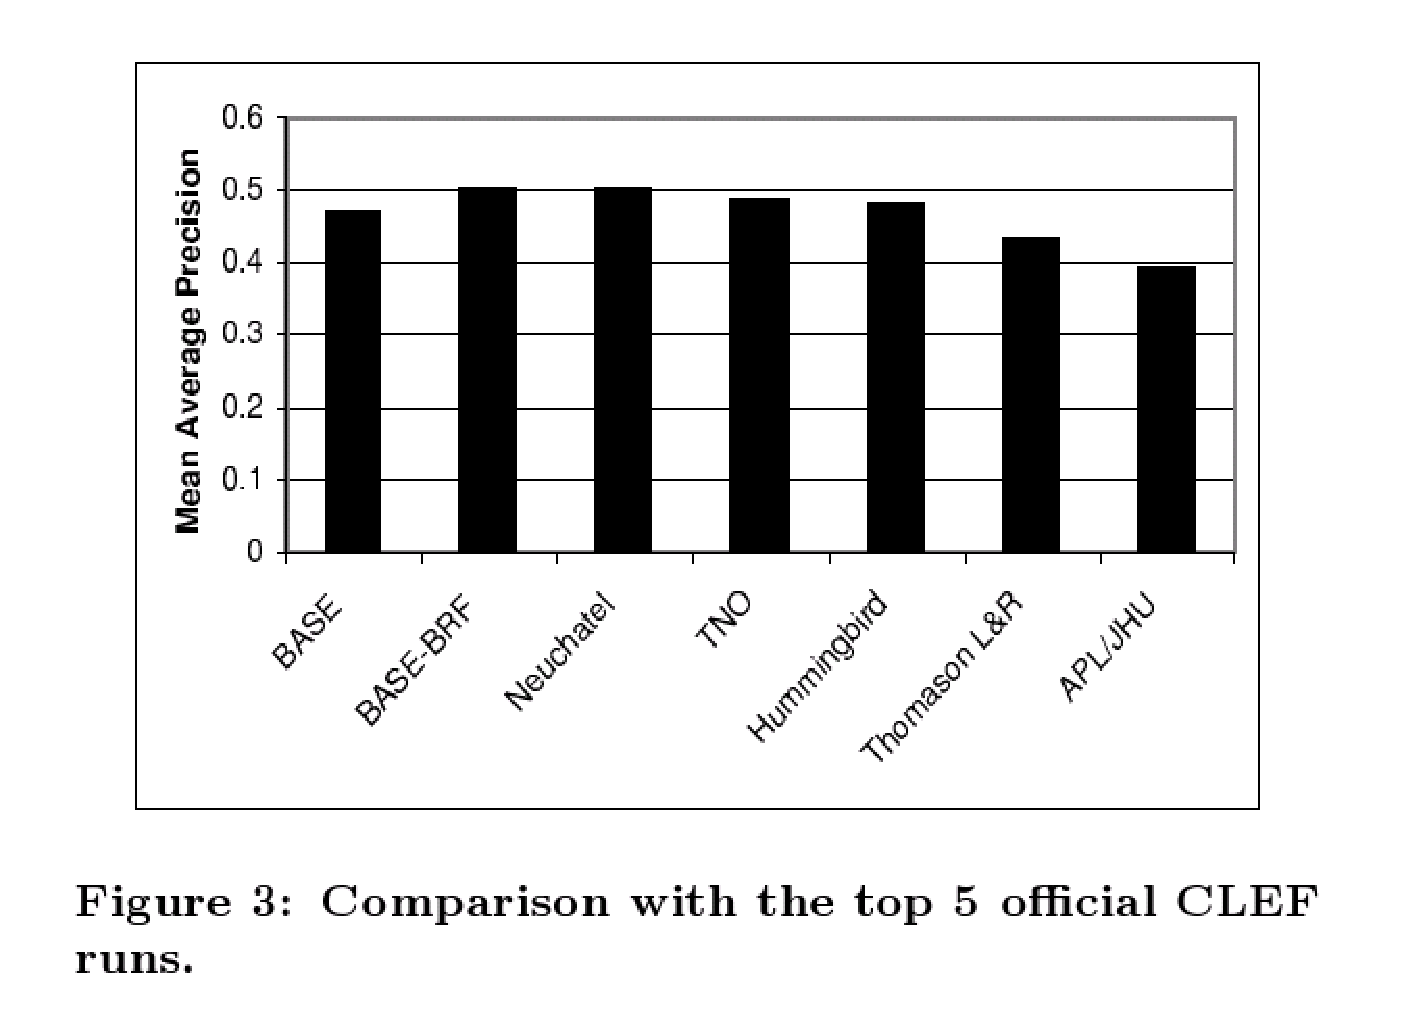
\includegraphics[width=\columnwidth]{fig/fig3}
  \end{figure}
}

\frame{
  \frametitle{Performance for English-French CLIR}
  \begin{figure}
    \centering
    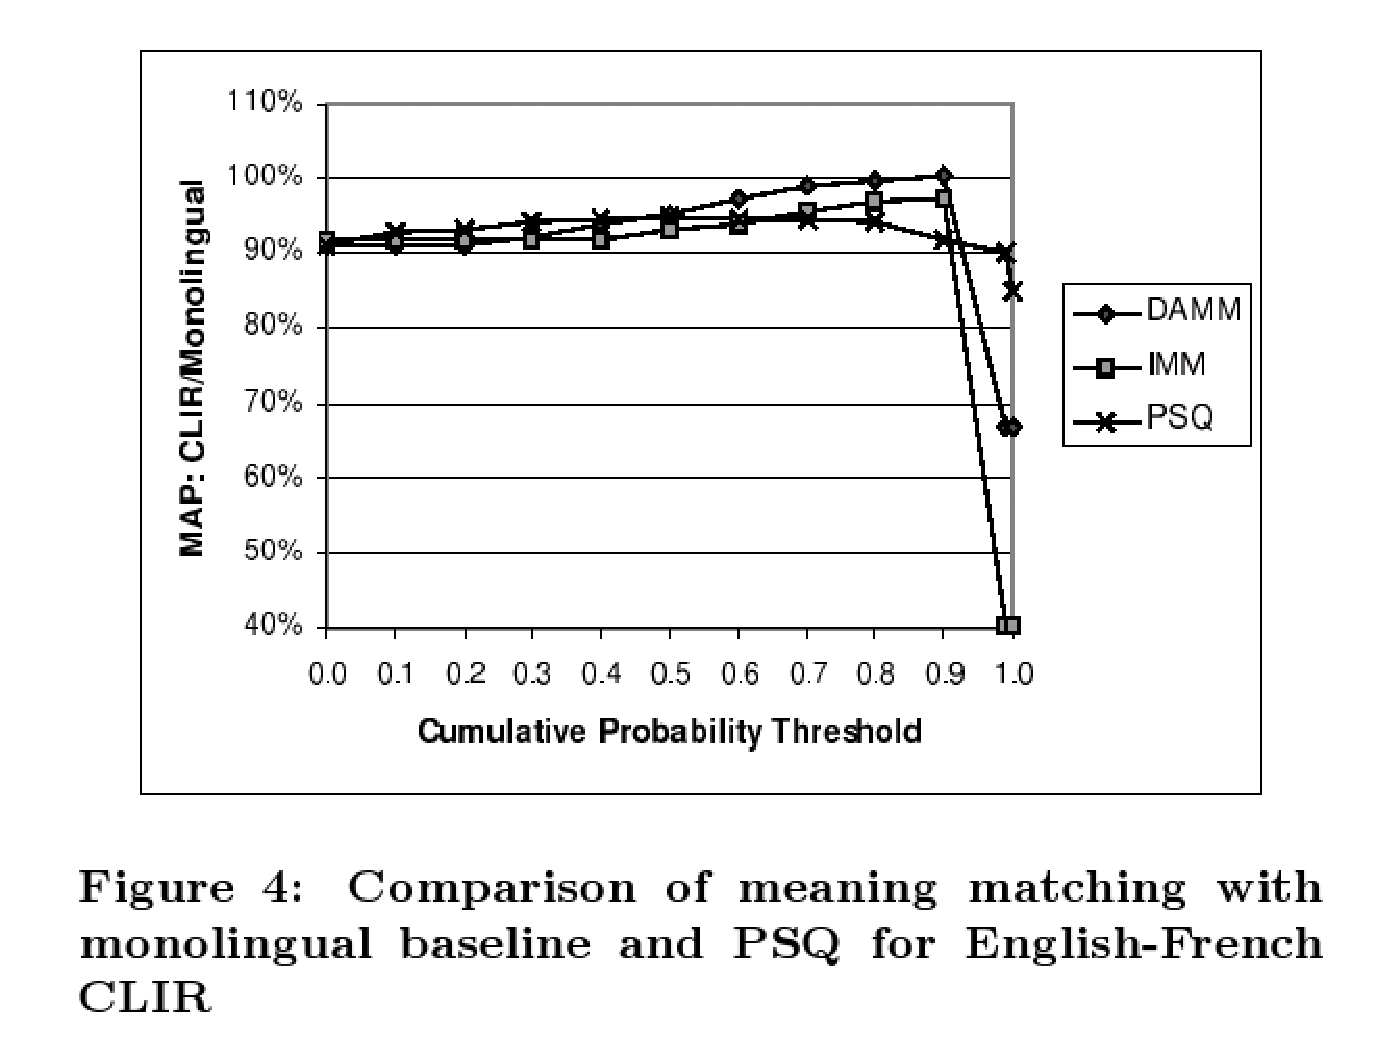
\includegraphics[width=\columnwidth]{fig/fig4}
  \end{figure}
}

\frame{
  \frametitle{Performance for English-Chinese CLIR}
  \begin{figure}
    \centering
    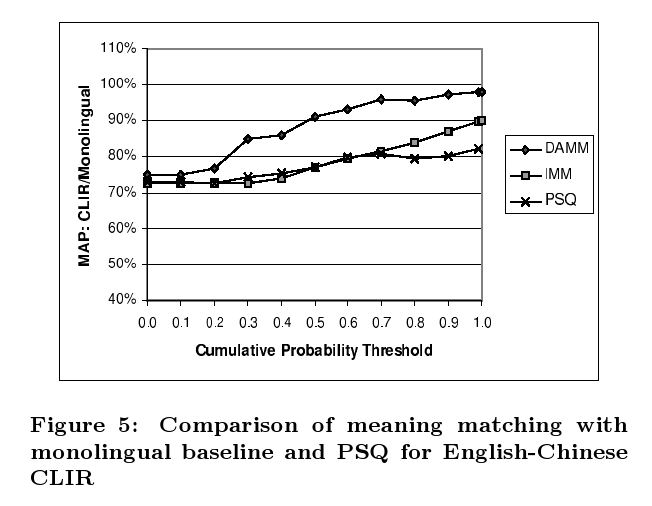
\includegraphics[width=\columnwidth]{fig/fig5}
  \end{figure}
}

\frame{
  \frametitle{Comparison between DAMM and PSQ}
  \begin{figure}
    \centering
    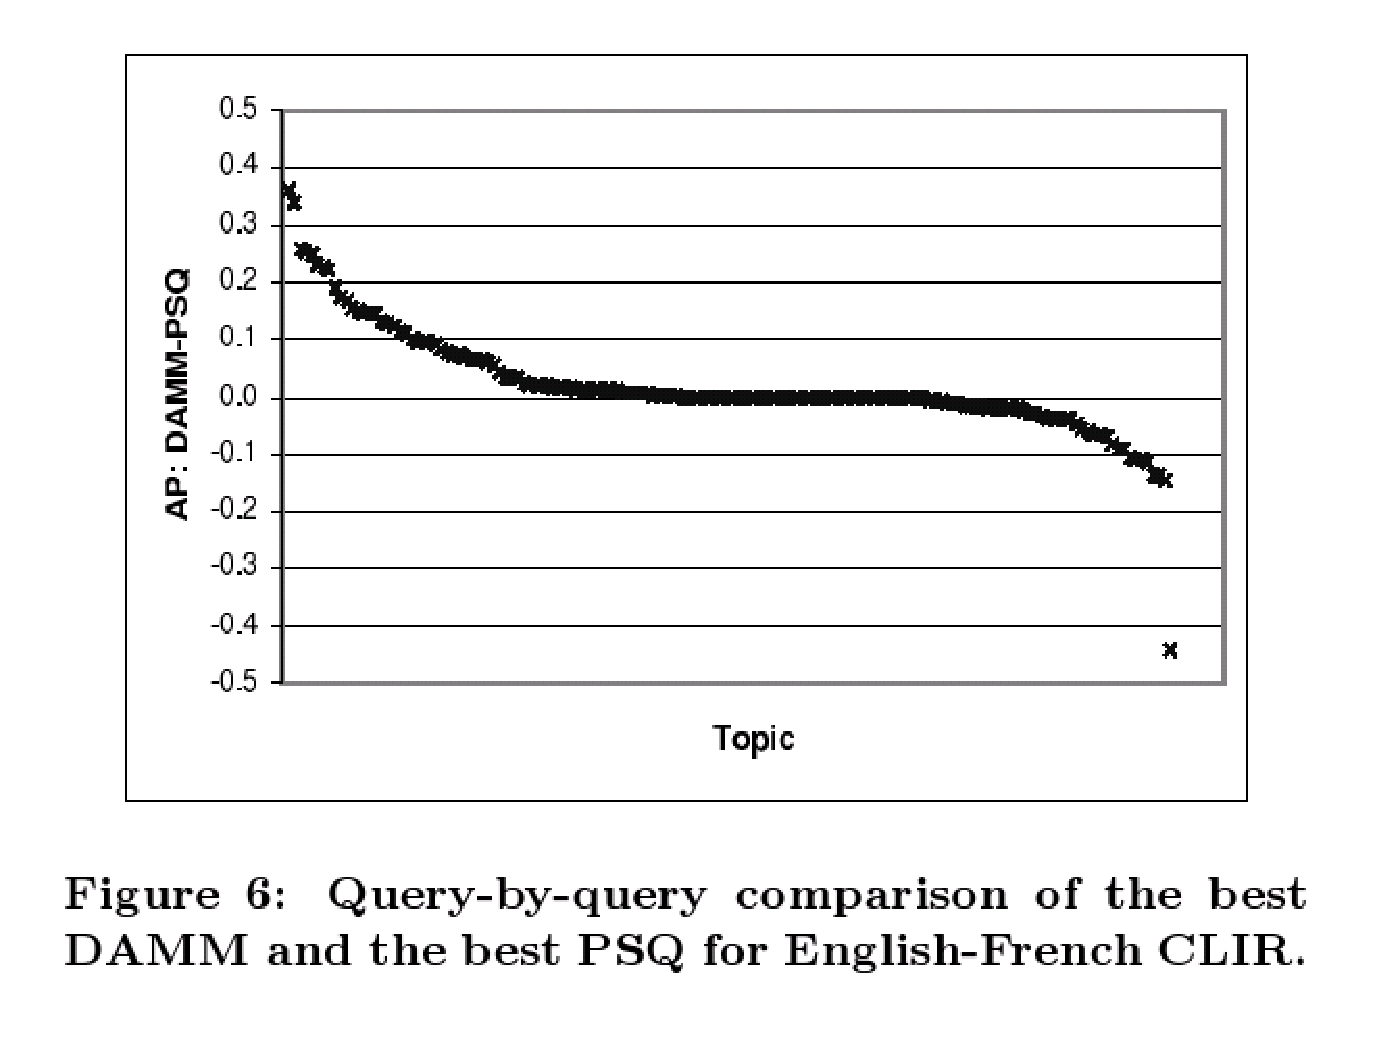
\includegraphics[width=\columnwidth]{fig/fig6}
  \end{figure}
}

\section{Conclusions}

\frame{
  \frametitle{Conclusions and Future Work}
  \begin{block}{Conclusion}
    \begin{itemize}
    \item A general framework for the use of translation probabilities in CLIR
    \item PSQ method as a special case of meaning matching model
    \item Significant improvement on CLIR performance
    \item Effective and robust meaning matching technique
    \end{itemize}
  \end{block}
  \begin{block}{Future Work}
    \begin{itemize}
    \item Phrasal translation
    \item Comparable corpora
    \item Parameter setting
    \end{itemize}
  \end{block}
}

% All of the following is optional and typically not needed. 
\appendix
\section<presentation>*{\appendixname}
\subsection<presentation>*{For Further Reading}

\frame{
  \frametitle<presentation>{For Further Reading}
    
  \begin{thebibliography}{10}
%--------------------------------------------------
%   \beamertemplatebookbibitems
%   \bibitem{Author1990}
%     A.~Author.
%     \newblock {\em Handbook of Everything}.
%     \newblock Some Press, 1990.
%-------------------------------------------------- 
    \beamertemplatearticlebibitems
    \bibitem{Braschler04}
      [Braschler04] Martin Braschler
      \newblock Combination approaches for multilingual text retrieval.
      \newblock In {\em Information Retrieval}, 7(1-2):183-204, 2004.
    \bibitem{Darwish03}
      [Darwish03] Kareem Darwish and Douglas W. Oard
      \newblock Probabilistic structured query methods.
      \newblock In {\em Proceedings of the 26th Annual International ACM SIGIR Conference on Research and Development in Information Retrieval}, pages 779-786, 2003.
  \end{thebibliography}
}

\frame{
  \frametitle<presentation>{For Further Reading (cont'd)}
  \begin{thebibliography}{10}
    \beamertemplatearticlebibitems
    \bibitem{Kang04}
      [Kang04] In-Su Kang, Seung-Hoon Na, and Jong-Hyeok Lee
      \newblock POSTECH at NTCIR-4: CJKE monolingual and Korean-related cross-language retrieval experiments.
      \newblock In {\em Working Notes of the 4th NTCIR Workshop}, National Institute of Informatics, 2004.
    \bibitem{McCarley99}
      [McCarley99] J. Scott McCarley
      \newblock Should we translate the documents or the queries in cross-language information retrieval?
      \newblock In {\em Proceedings of the 37th Annual Conference of the Association for Computational Linguistics}, pages 208-214, 1999.
  \end{thebibliography}
}

\frame{
  \huge
  Thank you!
}

\end{document}


